% Allow relative paths in included subfiles that are compiled separately
% See https://tex.stackexchange.com/questions/153312/
\providecommand{\main}{..}
\documentclass[\main/thesis.tex]{subfiles}

\iffalse
- Capturing and playing sound, digitally
- Representation (single frame vs multi(spectrum))
- Creating sound
    - Sound can be created functionally
    - sound can be created piece by piece 
- a quick history/summary of computer music technology (the parts of it that are relevant to our project)
    - Define vsts, synth parameters, filters, eqs since some they're involved in some of the previous works.
- Past work involving heuristic search and digital synths
- Past work involving generative neural nets
- Our work and how it's different or extends past work 
    - How it can be replicated
\fi

% todos:
% probably use amplitude and magnitude and power
% haven't described timbre 
% make reconstruction wave include multiple waveforms and how they go missing if sampling rate too slow
% haven't described nyquist frequency
    
\begin{document}

\chapter{Background and Related Work}

% AH: Digital Signals are a series of values (not digits) and 
%     perfectly valid way of saying a series of numbers.
%    

This chapter aims to provide a background for the subsequent chapters via a quick overview of three important topics: 
\begin{enumerate*}[label=(\roman*)]
  \item Digital sound, its features and concepts that have been fundamental to our work,
  \item  A quick overview of digital synthesis techniques, and
  \item Related works and their relative similarities and distinctions.
\end{enumerate*}
\section{Digital Audio: Sound from Numbers}
Sound is the result of a series of physical events. Most of what we hear is the product of physical disturbances, causing vibrations in our mutually shared, immersive mediums (air, hopefully). Sound waves carry these vibrations through air as part of an expanding, spherical wave front; Exponentially losing intensity as they travel away from the source \cite{cook1999chap4}. 
\\\\

[graph describing wave amplitude, phase and frequency here]
\\\\
A sound wave can be viewed as the result of a function which governs amplitude through time, where time and amplitude exist in continuous dimensions. Waves can be approximated via a series of samples, associating time steps to a discrete range of amplitude values. 
Given a wave generation method, computers can make sound by sending a series of discrete digits to a digital-to-analogue chip, which in turn can
create vibrations within a speaker.  \textit{Digital synthesis} of audio is the process of creating these discrete values. 
\\

\subsection{Sampling Rates and Quality of Digital Audio}
In 1963, Mathews wrote on the potential and utility of computers as digital instruments; By presenting a snapshot of digital audio technology of his time and making predictions on what would be possible in the future  \cite{mathews1963digital}. This work by Mathews makes the robust foundations of digital signal processing apparent as many of the techniques described have remained popular and relatively unchanged, yet subjected to up-scaling alongside Moore's law \cite{mack2011fifty,smith1991viewpoints}. For instance, Mathews described a general method for computers to capture and internally represent audio: By discretely sampling continuous pressure waves of sound and recreating the sound from numbers. 

As discussed previously, \ref{sec:computer make sound}, sound can take on the physical characteristics of a waveform. Imagine the curve shown in figure \ref{fig_sampling_rate} is representative of a sound wave we would like to digitally capture. As the sound travels through a microphone, its sensors can capture small packets of information about it. Each packet would represent the amplitude of the wave at a time-step. The more packets of information we get, the better our digital recreation of the original sound.

In this context, \textit{sampling rate}, is an important feature of digital sound, referring to the number of samples per second of audio (measured in Hertz, or Hz). Sampling rate is not the only important factor when recording audio as it is important to record the samples with not just speed, but also precision. Assuming perfect sensors, precision is the range of possible values we can assign to each sample. It is determined by bit depth: the number of bits we have to represent the values of each sample.  Today, standard quality audio often refers to sampling rates of 44.1 kHz and 48 kHz and bit depth of 16 (that's $2^{16}$ values), while "high quality" audio indicates an increase in bit rate or bit depth \cite{reiss2016meta}. Although subject to diminishing returns, high quality audio may be preferable to most musicians and audio-engineers; In a meta-analysis of digital sound perception, Reiss found a small but statistically significant portion of people are able to discriminate the effect of standard and high quality audio with no prior training, and a dramatically higher detection rate after extensive training~\cite{reiss2016meta}. 

% AH: please use word~\cite{author} not word \cite{author}

\begin{figure}[h]
\label{fig_sampling_rate}
\centering
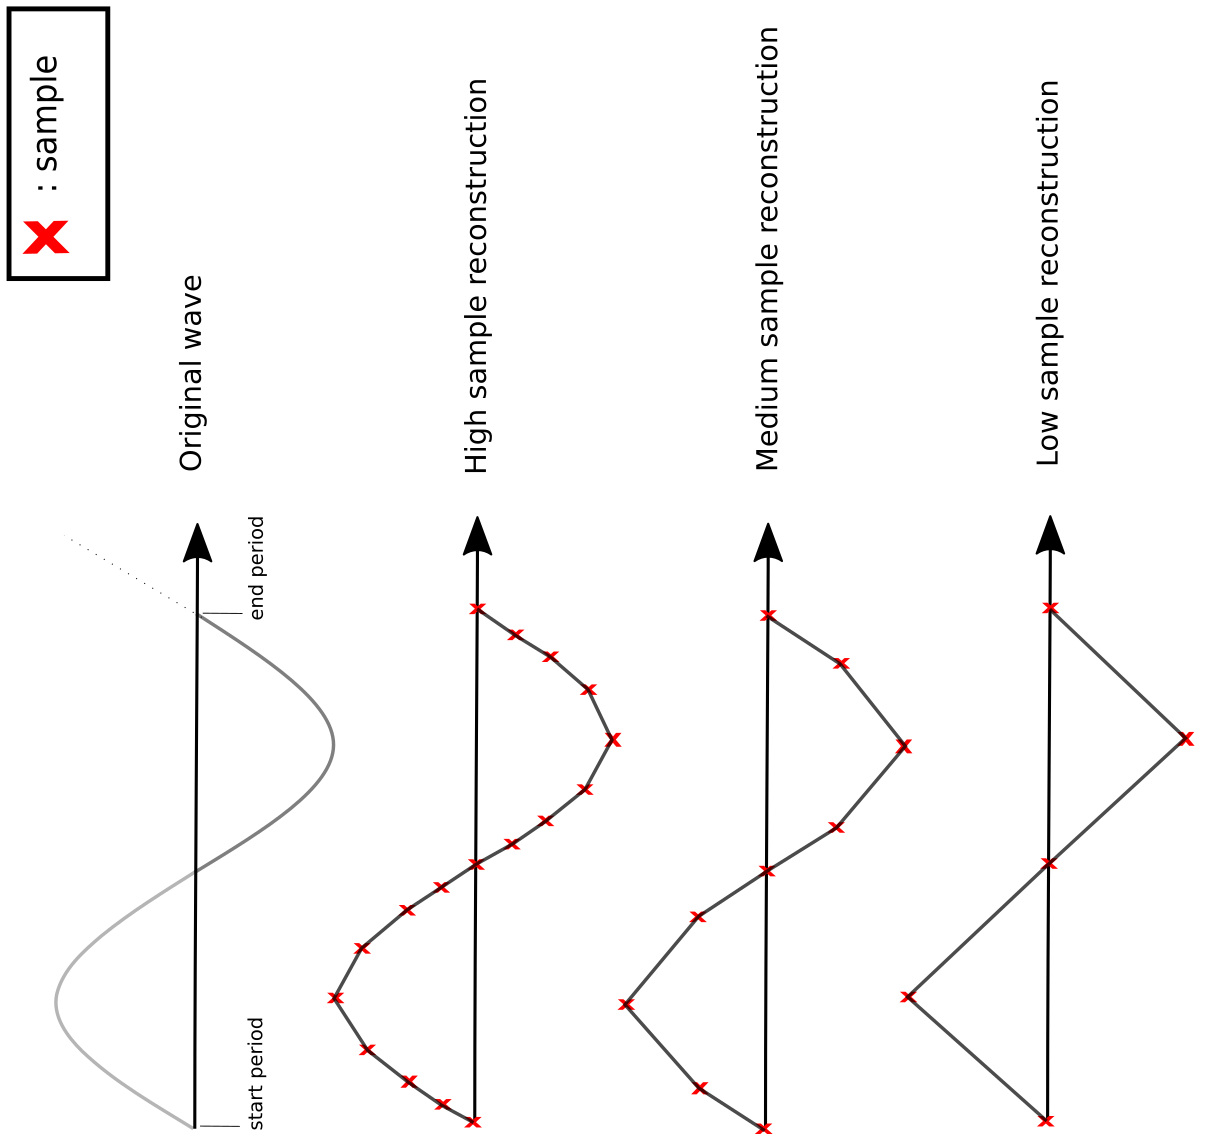
\includegraphics[width=1\linewidth,angle =-90 ]{images/periodic_function_decimation.png}
\caption{Reconstruction of a periodic, continuous wave at three different sampling levels. Higher sampling rates result in higher reconstruction accuracy. } % AH: this is linear interpolation many sound cards will convert the last signal back into the original wave just fine
\end{figure}

\\\\
\subsection{Loudness, Amplitudes and Envelopes}
Loudness is a subjective description of a sound's intensity or energy levels. It varies based on the complexity of sounds, the frequencies present, and hearing ability of the listener \cite{fletcher1933loudness,cook1999chap6}. It can only be measured relatively, by establishing a benchmark sound and surveying populations on the relative intensities \cite{cook1999chap6}. Since loudness and intensity of sound correlate with the amplitude of digital waveforms (the values assigned to the samples), an imperfect but convenient alternative method for inferring the the loudness of digital sounds is to compare relative amplitudes. 

\\
The peak level of a digital sound corresponds to the sample with the highest value. This method has its benefits, but leaves out an important factor: the duration of intensity. A more commonly used method of level detection is the Root Mean Square (RMS) method, which averages the values of a short sequence of samples for its calculation of levels.
\\
Sounds typically vary in intensity as they unfold. This change in intensity is often described by the "envelope" of the sound, particularly in shorter samples. For digital sounds, Mitchell describes the envelope as either (since samples typically take the range of -1 to 1) of the borders that are created by graphing a signal and connecting the local absolute peak values \cite{mitchell2009basicsynthChap6}. The envelope is generally described via 4 features: Attack, Decay, Sustain and Release (ADSR). Attack describes how quickly the peak loudness is reached. Decay for how quickly the sound drops to sustain level. Sustain is the duration of sustaining intensity (e.g how long a finger is kept on a piano key). Release describes the speed of fading to silence (e.g once a piano key is released).

Envelopes can be mathematically described and used to shape signals. A common approach in digital sound synthesis is to output all samples at a consistent amplitude and apply an envelope later down the synthesis chain. Digital and analog synthesizers often have built-in ADSR modules to shape the volume of the output and other parameters.  

[Graph of envelope shaping a signal]
% note: make sure you're using terms signal and waveform properly
\subsection{Frequency, Pitch and Spectrograms}
\textit{Frequency} is used to describe number of repetitions within a time-frame, or how frequently a cycle is repeated. The frequency of an audio signal is often measured in unit of hertz (cycles per second). Most sounds, particularly those from none virtual sources, are a combination of multiple different pressure waves with different frequencies and amplitudes. \textit{Pitch}, is a perceptual property of sound that is tied to the frequencies present in each sound. How we perceive and describe the pitch of a sound (e.g high-pitched vs low-pitched") is heavily dependent on the characteristics (frequency, amplitude, duration, etc) of the waveforms it contains. Some sounds such as piano chords or pure tones have easily discernable pitches. Others, such as "pink noise" or the sound of rain do not. Yet another factor to consider is the hearing ability of the subject, which varies between people based on factors such as age, environment, musical training, etc \cite{reiss2016meta,alain2007age,newman2012grm7}. 

Spectrograms are graphs used to showcase and analyze the duration and amplitude of frequencies present in a sound. Since we often do not have access to the time-variant systems behind sounds of interest, it is common to use function decomposition methods to break sounds down to a combination of simpler functions. A commonly used method for the breakdown of complex, time-variant functions is the fourier transformation and its variations. One such method is the discrete fourier transformation (DFT) and its inverse, often used to convert digital sound from its time domain representation (sequence of samples) to its frequency domain representation (sets of frequency ranges and their amplitude) and vice versa.\\\\

[spectrogram figures]
[figure of this breakdown]


% https://en.wikipedia.org/wiki/Frequency_domain#/media/File:Fourier_transform_time_and_frequency_domains_(small).gif

\section{Digital Audio Synthesis}

The phenomena of sound at intensities we commonly encounter can be described as a product of a \textit{linear system} of functions \cite{cook1999chap4}. A linear system is a system where the transformation of a overlapping inputs is equal to the sum of the separately transformed inputs \cite{lyons2004understandingChap1}. In a linear system $\mathcal{S}$ with valid inputs and outputs $x(i)$ and $y(i)$, if:

\begin{equation}
 \mathcal{S}(x(i_1)) \xrightarrow{generates} y(i_1)
\end{equation}
\begin{center}
    and
\end{center}
\begin{equation}
\mathcal{S}(x(i_2)) \xrightarrow{generates}y(i_2)
\end{equation}

The output of the system given both inputs is the sum of the individual outputs, or:
\begin{equation}
 \mathcal{S}(x(i_1)+x(i_2)) \xrightarrow{generates} y(i_1)+y(i_2) 
\end{equation}
\\
This concept has important implications digital audio creation and analysis. Simple tones can be combined to create complex sounds, and complex sounds can be broken down for easier analysis. It also allows systems based on experiments with simple sine waves to remain relevant in complex sound domains \cite{cook1999chap4}. \\\\
[graph of addition of two sine waves making a complex sine wave ]
\\

In their taxonomy of digital synthesis techniques, Smith defines four families of algorithms. Algorithms that process and modulate existing sounds (e.g granular synthesis, wavelets), Spectral models that aim to create a particular spectrum of sound (e.g additive, subtractive), physicals models which emulate the physics of real instruments (as discussed in section \ref{sec_tools_disposal}) and abstract models (e.g wave shaping, phase distortion) which for signal generation \cite{smith1991viewpoints}. 



\subsection{Filters, Oscillators...}
\subsection{?}
The rise of Digital Audio Workstations (DAW) \cite{leider2004digital} and Virtual Studio Technology (VST) based plug-ins \cite{tanev2013virtual} have rapidly transformed the sonic and material landscape of music production in the recent years. Coupled with this rise in popularity is a vast array of commercial products and services dedicated to satiating the need of amateur and professional music producers for unique sounds; most commonly via audio samples: one-shot drum samples, long sustained notes (commonly referred to as pads or textures), and loops (percussive or melodic) are common deliverables. Two notable examples of these commercial services are \textit{loopmasters}\footnote{loopmasters.com} and \textit{splice.com}\footnote{splice.com}. Furthermore, VST plug-ins can emulate complex audio synthesizers and effects which some producers may find daunting or time consuming to work with from scratch. In many cases VST plug-in vendors or unaffiliated enthusiasts sell additional presets for these plugins, targeted towards producers who do not have the time or interest in creating their own. The flexibility of the VST technology allows producers to further modify these presets until their desired sound is reached.

\section{Related Work and Contradistinctions}
\label{related}
Numerous deep, neural network models have been proposed and utilized for the purpose of signal generation in recent years. WaveGans and WaveNet have been subject to significant improvements and experiments since their proposal \cite{nsynth2017,yamamoto2019parallel,oord2017parallel}. Even more recently Variational AutoEncoders (VAE's) have been utilized for generation of short percussive samples \cite{aouameur2019neural,ramires2019timbfeat}. In this work however, we opt to use digital signal processing methods to create a virtual synthesizer for the generation of audio signals as it provides several unique advantages:
\begin{enumerate}[label=\roman*]
  \item Fast, offline rendering of audio with no reliance on GPU: Currently not possible with state of the art models such as parallel WaveGan \cite{yamamoto2019parallel} and parallel WaveNet \cite{oord2017parallel}. 
  \item Rendering at high sampling rates: Performance speed being a common issue, the standard sampling rate in most audio generation work utilizing neural networks appears to be under 24 khz \cite{yamamoto2019parallel,oord2017parallel,aouameur2019neural,ramires2019timbfeat}. However, a significant number of untrained human ears can detect a change in quality of audio between sampling rates of 192 khz and the industry standard of 44.1 khz \cite{reiss2016meta} with a dramatic increase in quality detection after training. Therefore we can safely assume that most producers would prefer their audio samples to have sampling rates of 44.1 khz or higher. In this work, we fix our sampling rate to the 48 khz standard. 
  \item Neural networks are often viewed as unexplainable black box solutions. Some models such as VAE's can learn an underlying latent space of parameters and capture the "essence" of the different labels in a dataset. However, these spaces are learned in an unsupervised manner and must be manually analysed, perhaps extensively, before they can be understood \cite{esling2018generative}. The use of a virtual synthesizer for audio generation makes our parameters readily understandable and easily modifiable. \\
\end{enumerate}

Automatic programming of virtual synthesizers has also been a topic of interest. In early 2000s, Interactive Genetic Algorithms (IGA's) were utilized for the generation of new sounds with various sound-engines \cite{johnson1999exploring,dahlstedt2001creating}. More recent work by Yee-King et al. \cite{yee2018automatic} used Long short-Term Memory (LSTM) models and genetic algorithms to find the exact parameters used to create a group of sounds. The sounds approximated were made by the same virtual synthesizer, not an external source; making the eventual replication certain even with random search. Since this work appears more focused on pads and textures rather than drums, feature matching appears to not be concerned with the envelope of the sounds but rather the frequency content within arbitrary time windows. Yet another recent, impressive work by Esling et al. used a large dataset of over 10,000 presets for a commercial VST synthesizer to learn a latent parameter space which can be sampled for creation of new audio \cite{esling2019universal}. As stated before, our work explores the rapid approximation of percussion sounds with no previous knowledge about the sonic capabilities of our virtual synthesizer, exploring the actual parameter space rather than its latent representation. 



\section{Data And Project Replication}
\label{data}

Our data is a large set of drum samples aggregated from personal libraries, free drum kits from the sample-swap project \footnote{https://sampleswap.org/} which we further processed to suit our categories, and a large set of drum sounds aggregated from royalty free sources such as musicradar \footnote{https://www.musicradar.com/}. We have made our dataset of free-drum sounds available for download. The scripts used to download and process royalty free samples will also be made available. Further information about downloading our dataset can be found on this project's github page. 

Our drum categories are claps, hats, kicks, rims/other, shakers, snares and toms. Other categories are chopped guitars, chopped pianos and n-stack-synths (random noise generated by the virtual synth with stack size of n, see \ref{vs}), utilized for learning percussive vs non-percussive sounds. Stack sizes refers to how many synth functions are connected together in a synthesizer.
Some notes about our dataset:


\begin{itemize}
\item Of the 6000 drum-sounds utilized in our work, the kick, snare and hat categories have the largest share at around 20\% each, while the shaker and rim (other) categories have the smallest at 5\% combined. Due to this we only focused on learning from kicks, snares, toms, claps and hats for Phase 1 of training (along with non-percussive groups of sound) \ref{sec:ear}.

\item For Phase 2 of training we only focused on categorizing snares, claps, kicks, hats and other (percussive sounds such as shakers, rims and unusual percussions that we couldn't categorize were grouped into this category). Non-percussive datasets were not used for this phase. 
\item In order to offset bias from data imbalance during training of our models, the categorical cross entropy loss was weighted by the group sizes. 
\item For any given model, 80\% of our data is used for training and 20\% is used for testing. 

\item We limit the size of the n-stack-synths category to 50\% of the total size of our drum dataset. This is done in order to measure whether the features extracted can address the "Open Set Recognition" problem, which will be discussed further in Section \ref{sec:ear}.
\end{itemize}
\end{document}